\section{Result 4: what a word means can be found in its row}\label{sec:probe}

Your idea starts from the claim that a model is a store of what words mean. In this language we
know exactly what each word means, so we can look for it inside a trained model. After training,
each animal has its own row of numbers in the word table. I asked two questions about the rows
of the nine models of the first round that had learned all 1,024 animals.

\textbf{Can a fact be read from a row?} I call this the read-out test. Take color. For each of
the four colors the test has a list of multipliers, one for each number in a row. It multiplies
each number of an animal's row by its multiplier and adds up the results; the color with the
largest total is its answer. The multipliers are worked out from half of the animals, whose
colors it is told. Then the test is tried on the other half, which it has never seen. If the
rows held no trace of color it would be right for about one animal in four.

\begin{table}[H]
\centering\small
\begin{tabular}{@{}rrrrrr@{}}
\toprule
Width & Color & Food & Home & Waking time & Facts shared with \\
 & & & & & the nearest row (of 4) \\
\midrule
8 & 71\% & 74\% & 70\% & 72\% & 3.98 \\
16 & 88\% & 84\% & 74\% & 83\% & 3.97 \\
32 & 97\% & 88\% & 97\% & 92\% & 3.98 \\
\bottomrule
\end{tabular}

\caption{Left four columns: how often the read-out test names the right value for animals it
was not worked out on, from their rows alone (average of the three repeats; guessing gives
25\%). Right column: how many of its four facts an animal shares with the animal whose row is
most like its own (two animals picked at random share 1.00).}
\label{tab:probe}
\end{table}

Table \ref{tab:probe} gives the result. The test is right for between 70\% and 97\% of the
unseen animals, far above guessing, and the wider the model the better. It is not right for all
of them, although the models themselves get every fact right. Either the rest is in the rows in a
form this very simple test cannot read, or part of it is kept in the body, which can tell an
animal by its row.

\textbf{Do animals with the same meaning sit together?} There are only 256 possible
combinations of four facts, and 1,024 animals, so nearly every animal has at least one other
animal with exactly the same four facts. For each animal I looked up the other animal whose
row is most similar: the one whose numbers are high where its own are high and low where its
own are low. Almost always it is one of those twins: the two share 3.97 or 3.98 of their 4 facts on average, where two animals
picked at random share 1. Nothing in the training text ever says that two animals are alike.
The model gave them nearly the same row because the same things are said about them.

\begin{figure}[H]
\centering
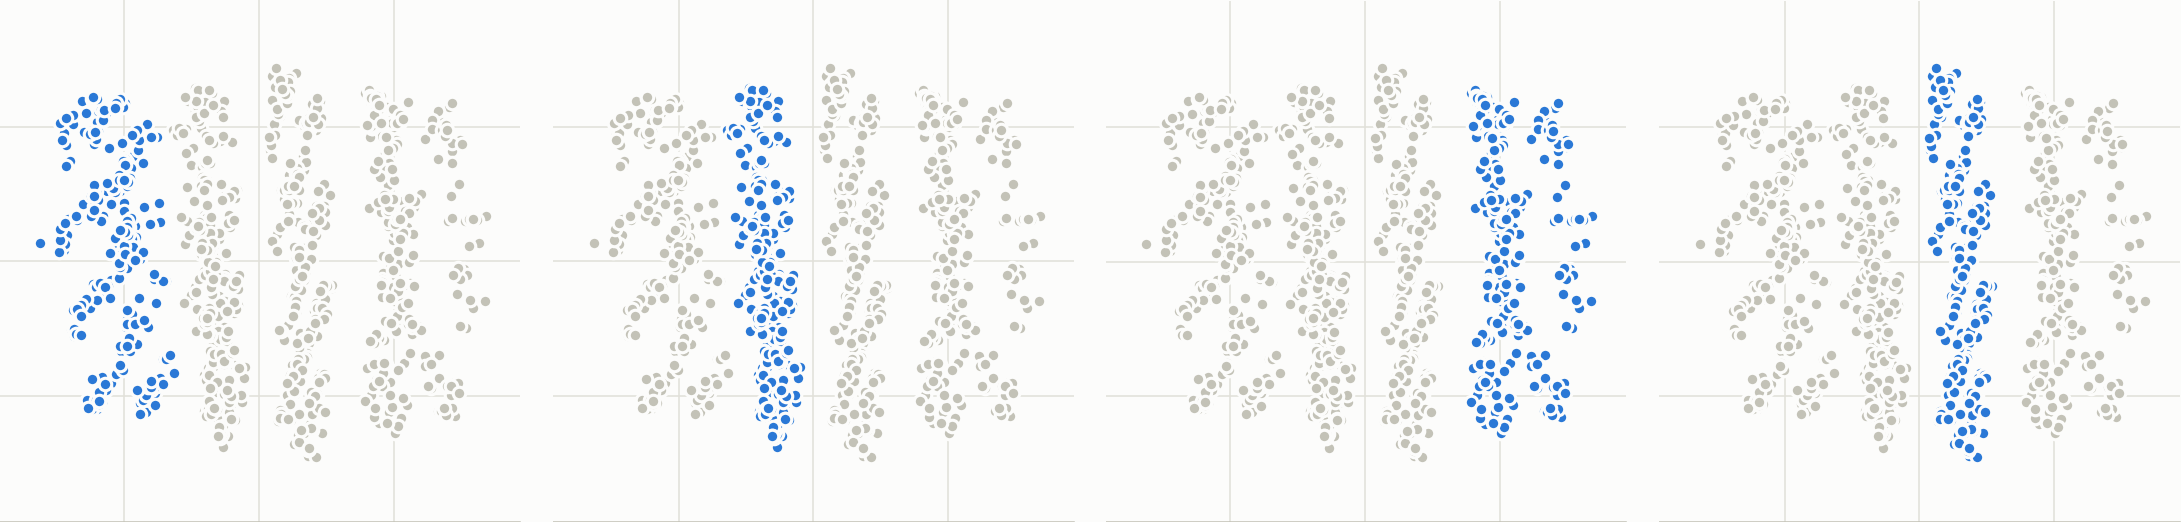
\includegraphics[width=0.74\textwidth]{figures/probe_strip.png}\\[1pt]
{\small\makebox[0.185\textwidth]{red}\makebox[0.185\textwidth]{brown}\makebox[0.185\textwidth]{green}\makebox[0.185\textwidth]{black}}
\caption{The rows of the 1,024 animals in one model of width 32. A row has 32 numbers, too many
to draw. So each row is squeezed down to two numbers, each a weighted sum of the 32, chosen as
the two sums that vary most from one animal to another. Each dot is one animal, placed by those
two numbers, so animals with similar rows land close together. The four panels show the same
dots; each colors in blue the animals of one color. They fall into four bands.}
\label{fig:probe}
\end{figure}

This supports the claim your idea starts from: in these models an animal's row is, to a large
extent, a description of what the word means. Animals that mean the same get nearly the same
row, and most of the meaning can be read out by a very simple test. It says nothing about size.
